\documentclass[12pt]{article}
%%%%%%begin preamble
\usepackage[hmargin=1in, vmargin=1in]{geometry} % Margins
\usepackage{hyperref}
\usepackage{url}
\usepackage{natbib}
\usepackage{graphicx}
\usepackage{amsmath}
\usepackage{amsfonts}
\usepackage{amssymb}
\usepackage{wrapfig}

\usepackage{multicol}
\usepackage{etoolbox}
%\patchcmd{\thebibliography}{\section*{\refname}}
%    {\begin{multicols}{2}[\section*{\refname}]}{}{}
%\patchcmd{\endthebibliography}{\endlist}{\endlist\end{multicols}}{}{}


\usepackage[normalem]{ulem}
\usepackage{xcolor}
\newcommand{\edit}[2]{\textcolor{purple}{\sout{#1} \textbf{#2}}}

\hypersetup{
  colorlinks   = true,
  %citecolor    = blue
  citecolor    = blue
  % gray is not being found!?!
  % gray is found if pdfpages is used... crap.
  %citecolor    = grey
  %citecolor    = Gray
}


%% headers
\usepackage{fancyhdr}
\pagestyle{fancy}
\fancyhf{} % sets both header and footer to nothing
\lhead{Evan H. Anders}
\rhead{Exeter Draft Rutherford Proposal}
\cfoot{\footnotesize{\thepage}}
%\pagestyle{empty}
%\pagenumbering{gobble}
%\renewcommand*{\thefootnote}{\fnsymbol{footnote}}

\renewcommand{\vec}{\ensuremath{\boldsymbol}}
\newcommand{\dedalus}{\href{http://dedalus-project.org}{Dedalus}}
\newcommand{\del}{\ensuremath{\vec{\nabla}}}
\newcommand{\scrS}{\ensuremath{\mathcal{S}}}

\newcommand{\prf}{Physical Review Fluids}
\newcommand{\ssr}{Space Science Reviews}
\newcommand{\araa}{Annual Reviews of Astronomy and Astrophysics}
\newcommand{\mnras}{Monthly Notices of the Royal Astronomical Society}
\newcommand{\aap}{Astronomy \& Astrophysics}
\newcommand{\apjl}{The Astrophysical Journal Letters}
\newcommand{\apj}{The Astrophysical Journal}

%\newcommand{\nosection}[1]{%
%  \refstepcounter{section}%
%  \addcontentsline{toc}{section}{\protect\numberline{\thesection}#1}%
%  \markright{#1}}
%\newcommand{\nosubsection}[1]{%
%  \refstepcounter{subsection}%
%  \addcontentsline{toc}{subsection}{\protect\numberline{\thesubsection}#1}%
%  \markright{#1}}

%\usepackage{atbegshi}
%%%%%%end preamble


%Make bibliography 2col
\bibliographystyle{apj_small}
\makeatletter
\renewenvironment{thebibliography}[1]
     {\begin{multicols}{2}[\paragraph*{\refname}\vspace{-0.1in}]%
      \@mkboth{\MakeUppercase\refname}{\MakeUppercase\refname}%
      \list{\@biblabel{\@arabic\c@enumiv}}%
           {\settowidth\labelwidth{\@biblabel{#1}}%
            \leftmargin\labelwidth
            \advance\leftmargin\labelsep
            \@openbib@code
            \usecounter{enumiv}%
            \let\p@enumiv\@empty
            \renewcommand\theenumiv{\@arabic\c@enumiv}}%
      \setlength{\itemsep}{-2pt}
      \sloppy
      \clubpenalty4000
      \@clubpenalty \clubpenalty
      \widowpenalty4000%
      \sfcode`\.\@m}
     {\def\@noitemerr
       {\@latex@warning{Empty `thebibliography' environment}}%
      \endlist\end{multicols}}
\makeatother



\begin{document}
\thispagestyle{fancy}
% Convection occurs in various places in nature. (no need for citation)
% There are interesting new observations of convection in blah blah blah (cite those, 2019, recent papers).
% A major problem in applied mathematics is coming up with theories that match these observations.
% In the next five years, I will use a combination of paper + pencil theory and numerical simulations to solve X problems (be a bit specific).
%^ that is the thesis sentence, think carefully about it.

Novel observations of convectively-driven flows in stars constantly prove that our theories of convection are incomplete.
For example, observations of massive stars demonstrate unexpectedly high mixing at the core convection boundary \citep{johnston_2021}, so theories underestimate the sizes of convective regions.
A recent observation has claimed the detection of waves driven by massive star core convection \citep{bowman_etal_2019}.
Such a wave signal could resolve disagreements about convective excitation mechanisms and the transfer of waves through stellar interiors \citep{rogers_etal_2013,lecoanet_etal_2021}.
Observations of the Sun show a convective conundrum: ``giant cells'' predicted by theory and simulations are not detected by many observations \citep{hanasoge&all2012,proxauf_2021}, suggesting that we do not understand the how the Sun's convection is driven.

A major problem in applied mathematics is developing theories that explain these observations.
In the next five years, \textbf{I will conduct research and create community tools to help resolve these and other modern mysteries in applied mathematics.}
%lead studies which help to resolve these discrepancies by improving theoretical models of convective boundaries, building community tools for studying the dynamical interiors of stars, and studying how the manifestations of fast processes like convection evolve over long, natural timescales.} 
People: Matt, Isabelle, 

% As mentioned in cover letter, mixing at convective interfaces is a major problem in astrophysics
% We think we have found the solution and we need to flesh out what the implications are.
% This is going to be great for a PhD student to work on, because we basically already know the answer 
% Safe papers, high impact. (don't use term safe papers)
\paragraph*{Task 1: Convective boundary mixing}
As I mentioned in my cover letter, mixing at convective interfaces is a compelling problem in astrophysics.
My recent work on penetrative convection may help to resolve discrepancies between observations and theory \citep{anders_etal_2022a}.
My previous work focused on a minimal model: it employed the incompressible Boussinesq approximation, and it studied a Cartesian domain.
There remains a great deal of work to be done in developing a robust theory of penetrative convection that works broadly in stellar evolution.
For example, the effects of rotation, composition gradients, magnetic fields, density stratification, and geometry have not yet been studied in detail.
Furthermore, use of the fully compressible equations subtly changes the theoretical constraint that I derived, and must be explored.
%Studying penetrative convection in the presence of any of these complications would be an excellent PhD project.
%We already know the zeroth order answer of how this process works, so there is a solid foundation for students to build upon, and because the stellar modeling community is invested in this work, it will give students a meaningful and high-impact way to contribute in the field.

Need to mention COBOM erc stuff that Isabelle has done.
Mention that this is a \emph{complementary} approach; Here I focus on long term evolution and saturation; they focus on rare event statistics; put these together and boom.
Matt's expertise in dissipation modeling.

\begin{wrapfigure}{r}{0.3\textwidth}
	\begin{center}
	\vspace{-10pt}
    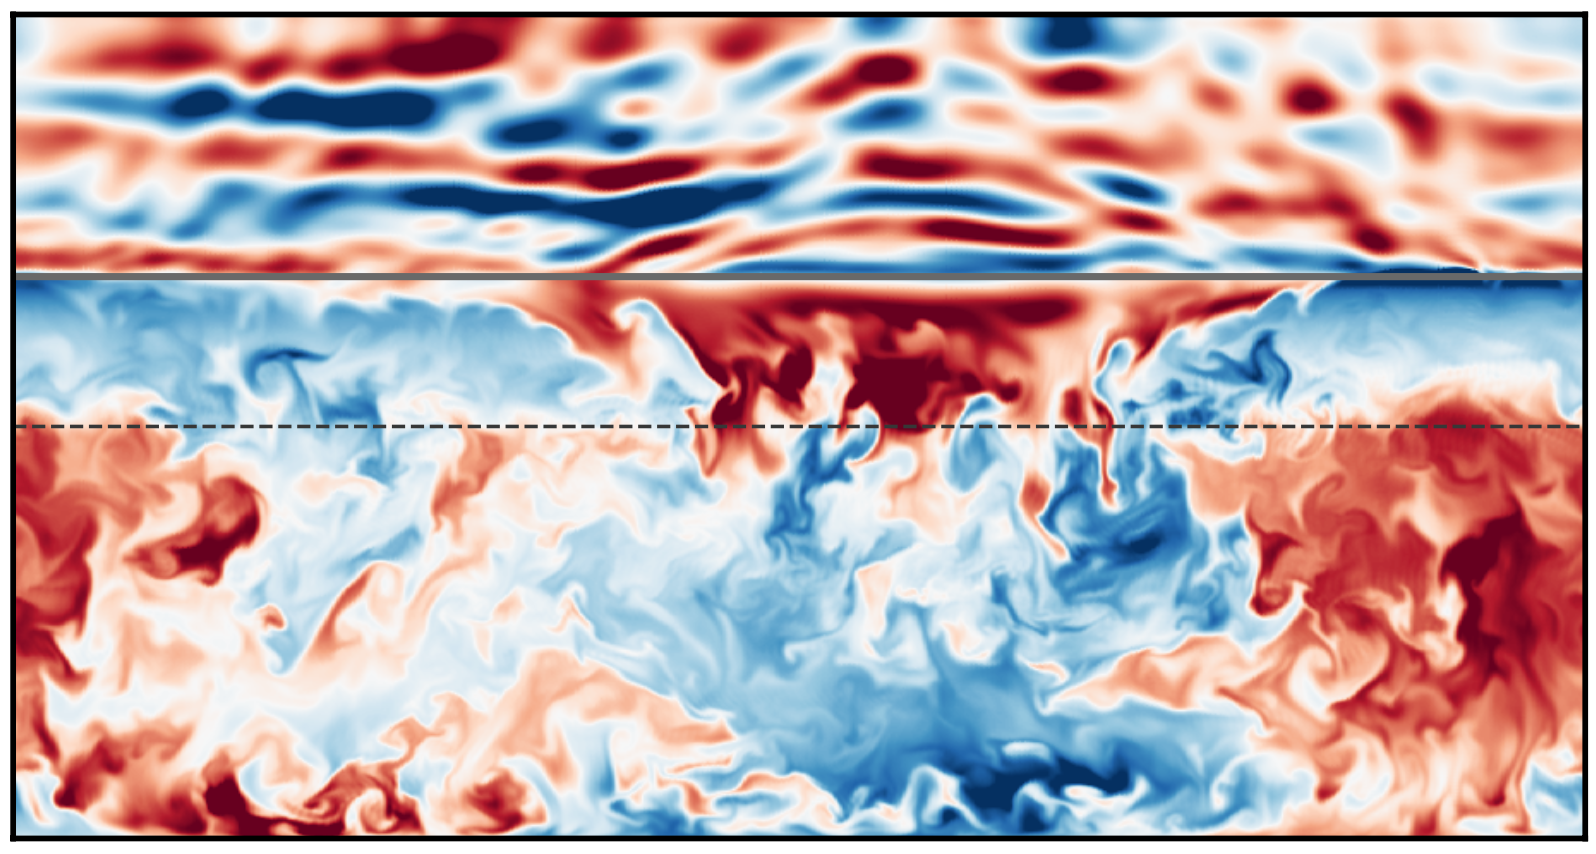
\includegraphics[width=0.28\textwidth]{./figs/penconv.png}
	\vspace{-16pt}
	\end{center}
    \caption{ A vertical slice of the temperature anomaly in a 3D simulation of penetrative convection.
	\label{fig:penconv} }
\end{wrapfigure}




%Get less convection-y
%Problem: ease of access. Right now there are no open-source codes for running convection simulations using realistic stellar structure models (Rayleigh uses a part of the model; it's not doing the full physics)
%Although convection is very important in stellar astrophysics, there are few tools available for running multi-D stellar astrophysics codes in realistic environments.
%I will make a version of the dedalus code / a software framework where users can directly import a stellar structure model (e.g., from MESA) and directly solve the fluid dynamics equations (MHD, hydro, anelastic, fully compressible) from the center of the star to its surface or a specified subset of the star's radius.
%I have run bespoke simulations that are useful for studying specific problems, but it is not something that non-experts could do readily. These are the challenges that come in from doing this: list.
%But I will solve these issues and make this great thing that everyone is going to be using.
%The point: being able to run verified stellar convection simulations in dedalus easily.
\paragraph*{Task 2: Open-source, easily accessible code for multi-D stellar simulations}
There are no open-source, user-friendly codes for running dynamical simulations of stars.
Current stellar dynamics codes require help from an expert to run, are restricted to limited equation sets, or only focus on a portion of the stellar domain.
Over the next five years, I will build an easy-to-use Python module that uses the Dedalus pseudospectral framework \citep{burns_etal_2020} to create dynamical simulations of full stars.
It is possible to include the full stellar domain in Dedalus, because flows that pass through the coordinate singularity at $r = 0$ can be resolved \citep{vasil_etal_2019, lecoanet_etal_2019}, and radial discretization can be fine-tuned so that resolution elements are localized in turbulent regions.
Background stellar stratifications will be imported from MESA stellar models \citep{paxton&all2011}.
Planned evolutionary equation sets will include both hydrodynamic and magnetohydrodynamic formulations of both the anelastic and fully compressible equations.
All of these formulations must be verified in the various dynamical regimes occurring in stars.
I will need to build a robust scheme for radial discretization that handles arbitrary stars at various stages in stellar evolution.
My 7 years of experience using Dedalus has given me the expertise to implement and debug all of these features.
Once complete, my proposed open access module will enable researchers to carry out experiments to understand observations like those discussed in my introduction.

Need to be careful here and mention that Matt will be crucial due to his expertise with Massive star simulations (but with a core boundary condition) and Isabelle's experience with music and envelope convection.

\begin{wrapfigure}{r}{0.3\textwidth}
	\begin{center}
	\vspace{-10pt}
    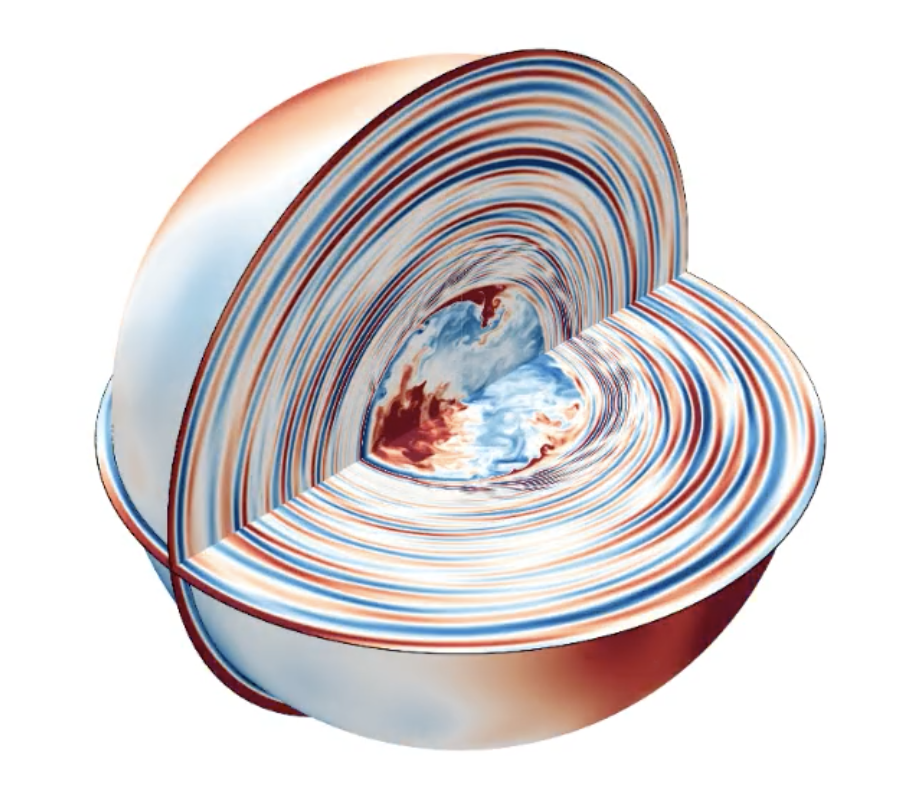
\includegraphics[width=0.28\textwidth]{./figs/massive_star.png}
	\vspace{-16pt}
	\end{center}
    \caption{ A volume rendering of scaled entropy fluctuations in a Dedalus simulation of a 40 $M_\odot$ star.
	\label{fig:massive_star} }
\end{wrapfigure}



\paragraph*{Task 3: The parameter space of convection}
Running simulations of stellar convection is difficult, because something is idealized.
This idealization can throw off the detailed force balances felt by the convective flows in unexpected ways.
In the fully constrained regime we generally understand what happens.
However in the transitional regime it's less clear (predictive rossby).
I will study simulations of rotating convection in a solar-type star and measure the force balances directly and determine how the rossby number scales as a function of stratification, convective driving, and rotation rate.


\paragraph*{Task 4: Convection at the smallest scales}
What is the convective conundrum.
What is the entropy rain hypothesis.
What did we learn in our previous entropy rain paper.
What work is left to do on the thermal model of entropy rain.
What work is left to do on the plume model of entropy rain. (tarshish, romps).

\begin{wrapfigure}{r}{0.3\textwidth}
	\begin{center}
	\vspace{-10pt}
    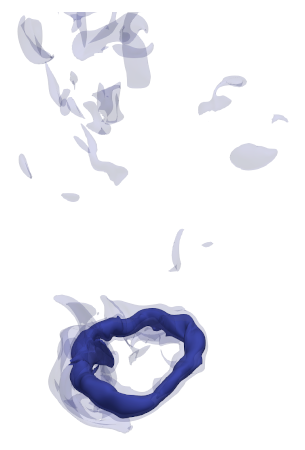
\includegraphics[width=0.28\textwidth]{./figs/turbulent_thermal.png}
	\vspace{-16pt}
	\end{center}
    \caption{ A volume rendering of an evolved thermal in its buoyant vortex ring state.
	\label{fig:massive_star} }
\end{wrapfigure}



%\paragraph*{Problem 3: Discrepant timescales}
%Convection includes both short timescales associated with turbulent motions and long timescales associated with, for example, the restratification of the background state.
%Discrepant timescales such as these occur in a variety of natural contexts, making it difficult to understand the long-term evolution of natural systems.
%For example, in stars, the rate at which nuclear burning changes is very slow compared to any dynamical process (convection, wave propagation, rotation, magnetic dynamo cycle, etc.).
%Understanding how short and long timescale processes nonlinearly interact is crucial for minimizing computational cost and ensuring robust results, because simulations of turbulent flows can only compute a few tens or hundreds of dynamical timescales.
%I have examined how fast and slow processes affect one another in the context of convection, and I would like to create a general framework for understanding how processes operating on discrepant dynamical timescales interact in natural systems.
%%Methods that I used to understand interactions between the convective overturn timescale and the thermal relaxation timescale could be applied to, e.g., 
%Slowly-evolving phenomena that are influenced by fast dynamics include, for example, latitudinal differential rotation profiles in rotating convection simulations, the evolution of shear flows via Reynolds stresses, and the evolution of large-scale magnetic fields in dynamo simulations.
%Studying methods for accelerating the evolution of any of these phenomena would make an excellent PhD project.


%\paragraph*{Beyond Research}
%I love teaching and am excited to teach any of the undergraduate mathematics or physics courses offered by the School. 
%As for graduate education, my research background has best prepared me to lead the Theoretical Physics ``Computational Research Skills in Physics'' MRes module or to mentor a research component under the ``Astrophysics and Geophysics'' theme.
%I currently co-mentor five graduate students, and have co-mentored undergraduate students in the past; I look forward to starting a vibrant research group where PhD, MRes, and undergraduate students all feel welcome, and where individuals whose identities are underrepresented in mathematics, physics and astrophysics can build confidence and identities as people in STEM.
%When I was a graduate student at the University of Colorado, I created and iterated upon the first rubric used in the graduate admissions process to make it more equitable and I would love to work on similar processes at Newcastle.
%As a postdoctoral fellow at CIERA, I chaired a public outreach committee for a year and have been actively involved in organizing a climate survey for the 2022-2023 academic year.
%I enjoy working to make my department a more fair, equitable, and just place, and I will bring this dedication and drive with me to Newcastle.

{\scriptsize
\bibliography{biblio}
}
\end{document}
